%%%%%%%%%%%%%%%%%%%%%%%%%%%%%%%%%%%%%%%%%%%%%%%%%%%%%%%%%%%%%%%
%
% Welcome to writeLaTeX --- just edit your LaTeX on the left,
% and we'll compile it for you on the right. If you give 
% someone the link to this page, they can edit at the same
% time. See the help menu above for more info. Enjoy!
%
%%%%%%%%%%%%%%%%%%%%%%%%%%%%%%%%%%%%%%%%%%%%%%%%%%%%%%%%%%%%%%%

% --------------------------------------------------------------
% This is all preamble stuff that you don't have to worry about.
% Head down to where it says "Start here"
% --------------------------------------------------------------
 
\documentclass[14pt]{article}
 
\usepackage[margin=0.5in]{geometry} 
\usepackage{amsmath,amsthm,amssymb}
\usepackage{graphicx}
\usepackage{hyperref}
\usepackage{color,soul}
\usepackage{caption}
\usepackage{courier}
\usepackage{listings}
\usepackage{xcolor} % for setting colors


\newcommand{\N}{\mathbb{N}}
\newcommand{\Z}{\mathbb{Z}}
 
\newenvironment{theorem}[2][Theorem]{\begin{trivlist}
\item[\hskip \labelsep {\bfseries #1}\hskip \labelsep {\bfseries #2.}]}{\end{trivlist}}
\newenvironment{lemma}[2][Lemma]{\begin{trivlist}
\item[\hskip \labelsep {\bfseries #1}\hskip \labelsep {\bfseries #2.}]}{\end{trivlist}}
\newenvironment{exercise}[2][Exercise]{\begin{trivlist}
\item[\hskip \labelsep {\bfseries #1}\hskip \labelsep {\bfseries #2.}]}{\end{trivlist}}
\newenvironment{problem}[2][Problem]{\begin{trivlist}
\item[\hskip \labelsep {\bfseries #1}\hskip \labelsep {\bfseries #2.}]}{\end{trivlist}}
\newenvironment{question}[2][Question]{\begin{trivlist}
\item[\hskip \labelsep {\bfseries #1}\hskip \labelsep {\bfseries #2.}]}{\end{trivlist}}
\newenvironment{corollary}[2][Corollary]{\begin{trivlist}
\item[\hskip \labelsep {\bfseries #1}\hskip \labelsep {\bfseries #2.}]}{\end{trivlist}}

\newenvironment{solution}{\begin{proof}[Solution]}{\end{proof}}
\newenvironment{courier}{\ttfamily}{\par}

% set the default code style
\lstset{
    frame=tb, % draw a frame at the top and bottom of the code block
    tabsize=4, % tab space width
    showstringspaces=false, % don't mark spaces in strings
    numbers=left, % display line numbers on the left
    commentstyle=\color{orange}, % comment color
    keywordstyle=\color{blue}, % keyword color
    stringstyle=\color{red} % string color
}

\begin{document}
 
% --------------------------------------------------------------
%                         Start here
% --------------------------------------------------------------
 
\title{\textbf{Brief Document On the Hall C Coincidence Time Physics Module}}%replace X with the appropriate number
\author{Carlos Yero} %if necessary, replace with your course title
 
\maketitle
\noindent The Hall C Coincidence Time Physics Module, THcCoinTime.cxx(.h), was created to facilitate the analysis of
coincidence time data by adding coincidence time variables to the ROOT Tree, so that users may apply any
cuts they desise to clean-up the data. This document intends to briefly cover what was done in physics module,
as well as the mathematical background, which was written by Latif Kabir during the start of Commissioning in 2018.\\

\section{Discussion on the Physics of Coincidence Timing}
The coincidence time measured between two spectrometers is defined as the time difference between the
two single-arm spectrometer triggers. The time difference is determined using the raw (uncorrected) TDC times,
therefore, additional corrections will be needed to reduce the natural spread in the coincidence peak.
As pointed out in Latif's paper, the corrections are as follows:
\begin{enumerate}
\item The leading order correction is the time taken by the partilcle to arrive at the focal plane following the
  central path, $L_{0}$, of the spectrometer.
\item The second order correction is due to the fact that the particle may not necessarily follow the central path, therefore,
  the time difference between particle path and central path, $\Delta L$, needs to be accounted for.
\item The third order correction is the fluctuations in the focal plane time with respect to the central time.
\item The last correction has more to do with a general offset of the coincidence peak, rather than an effect on the
  resolution. The peak is typically shifted to zero, to represent the occurrence of a true coincidence event originating
  from the same electron beam bunch.
\end{enumerate}
The raw coincidence times in the physics module were mathematically expressed as
\begingroup
\normalsize
\begin{equation}\label{eq1}
t_{\text{coin, raw}} = (t_{\text{SHMS, raw}} + t_{\text{SHMS, fp}}) - (t_{\text{HMS, raw}} + t_{\text{HMS, fp}})
\end{equation}
\endgroup

\noindent where the focal plane times were included as a correction to the raw tdc trigger times to simplify calculations later on.
The corrected coincidence time can then be expressed as
\begin{equation}\label{eq2}
t_{\text{coin, corr.}} = t_{\text{coin, raw}} \pm (t_{\text{elec. corr}} - t_{\text{hadron corr.}}) - \delta_{\text{offset}}
\end{equation}
where the sign convention is
\[ \text{sign} =
  \begin{cases}
    +  &  \text{SHMS (hadrons), HMS (electrons)}\\
    -  &  \text{SHMS (electrons), HMS (hadrons)}
  \end{cases}
  \]
  \noindent The sign depends on the particle type the spectrometer is set to detect, as we want to ensure the correction is \textit{subtracted off}
  from the right spectrometer raw trigger time. For example, if the SHMS is set to detect electrons, then substituting Eq. \ref{eq1} in Eq. \ref{eq2}, one obtains
  \begin{equation}\label{eq3}
    \begin{aligned}
      t_{\text{coin, corr.}} & = (t_{\text{SHMS, raw}} + t_{\text{SHMS, fp}}) - (t_{\text{HMS, raw}} + t_{\text{HMS, fp}}) - (t_{\text{elec. corr}} - t_{\text{hadron corr.}}) - \delta_{\text{offset}} \\
                          & = (t_{\text{SHMS, raw}} + t_{\text{SHMS, fp}} - \text{\textcolor{red}{$t_{\text{elec. corr}}$}}) - (t_{\text{HMS, raw}} + t_{\text{HMS, fp}} - \text{\textcolor{red}{$t_{\text{hadron corr.}}$}})  - \delta_{\text{offset}}
    \end{aligned}
    \end{equation}  
  \noindent By subtracting the electron/hadron timing corrections, the dependence on the particle pathlength and beta, $\beta$, are
  removed. Therefore, if a \textit{true} coincidence occurs, it will land at the same location in the coincidence timing spectrum, regardless
  of the particle type. See Figure \ref{fig:eH_Coin}. \\ \newline
  \begin{figure}
  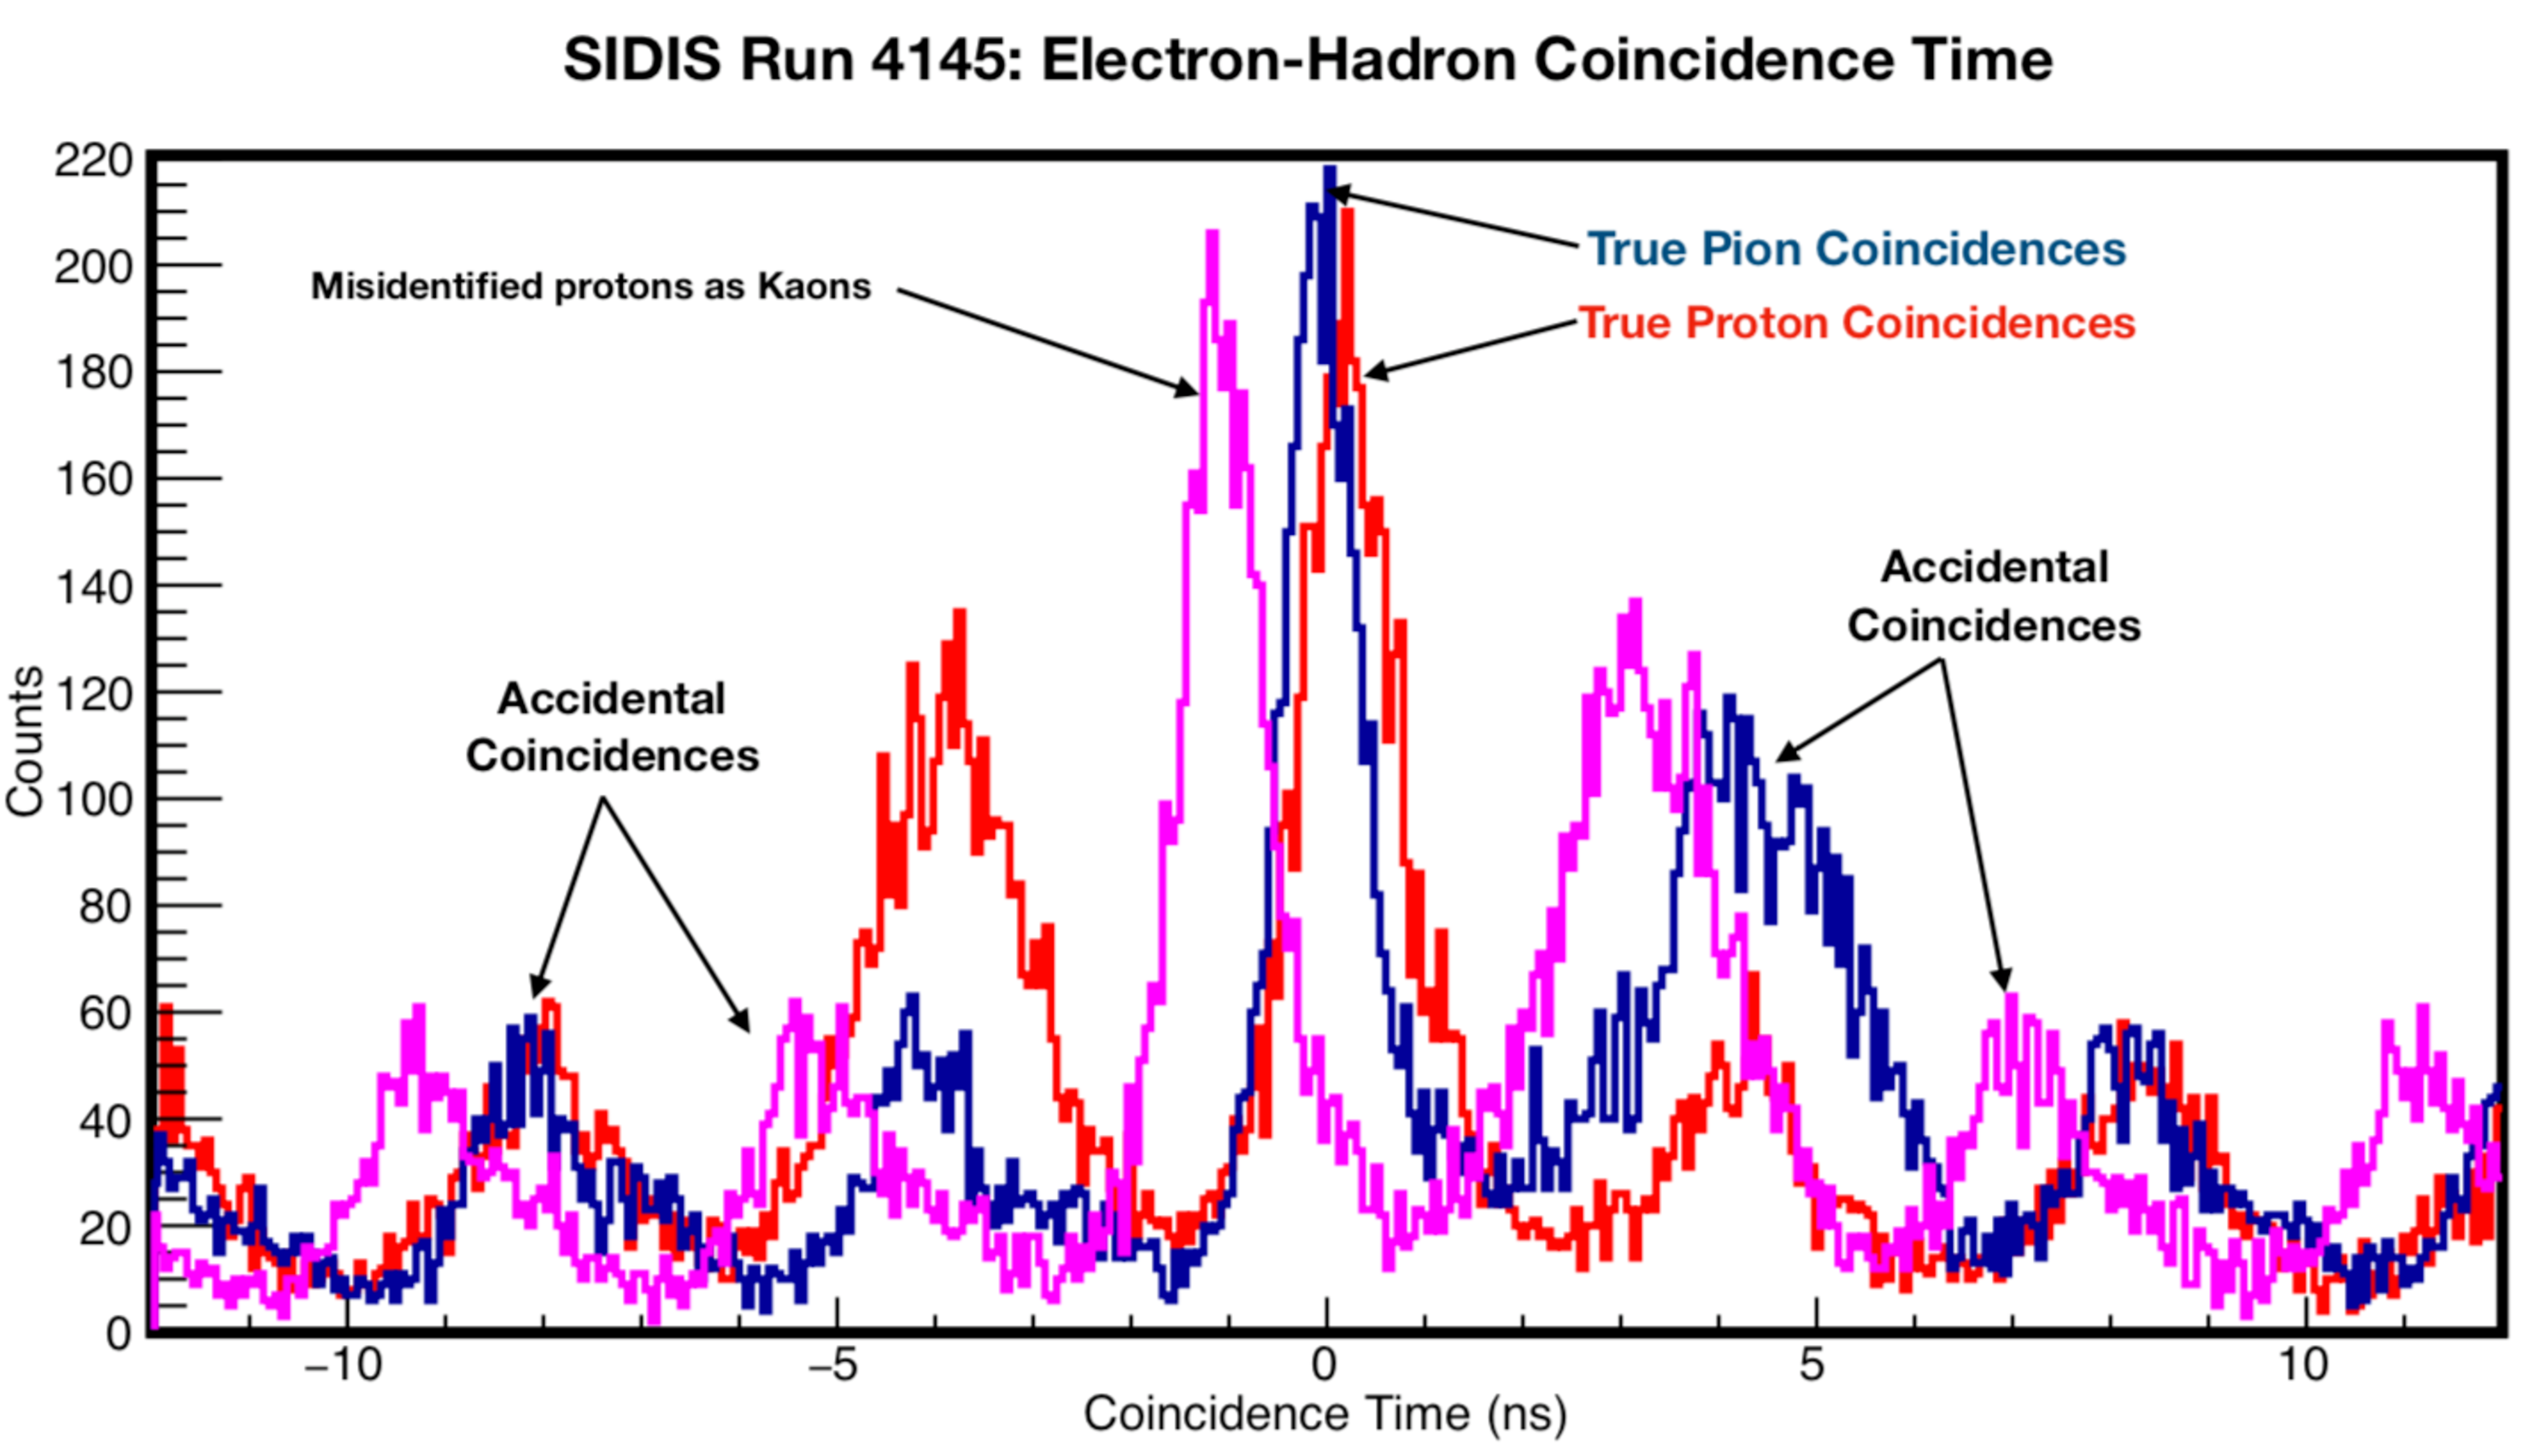
\includegraphics[scale=0.3]{eH_Coin.pdf}
  \caption{Electron-hadron coincidence time, assuming proton, $\pi^{+}$ and K$^{+}$ mass.}
  \label{fig:eH_Coin}
  \end{figure}
  \noindent The timing corrections for electrons and hadrons in Eq. \ref{eq3} can be expressed in the general form
  \begin{equation}
    \begin{aligned}
      t_{\text{e(h) corr.}} = \frac{L_{0} + \Delta L}{\beta c}, \text{  where } \beta \equiv \frac{p}{E} = \frac{p}{\sqrt{m^{2} + p^{2}}}
    \end{aligned}
  \end{equation}
  The variables ($L_{0}$, $\Delta L$) are the 1st and 2nd order path length corrections, corresponding to either the HMS or SHMS, depending on which particle
  is assigned to which spectrometer. The variable $\beta$, represents
  the particle fractional velocity relative to the speed of light, and depends on the particle mass and momentum. Therefore, subtracting off all these
  dependences from the raw coincidence time, places the coincidence peak at a certain offset, $\delta_{\text{offset}}$, which can then be determined experimentally, and
  shifted to zero (0 ns). (See Figure \ref{fig:eH_offset})
  \begin{figure}[h]
  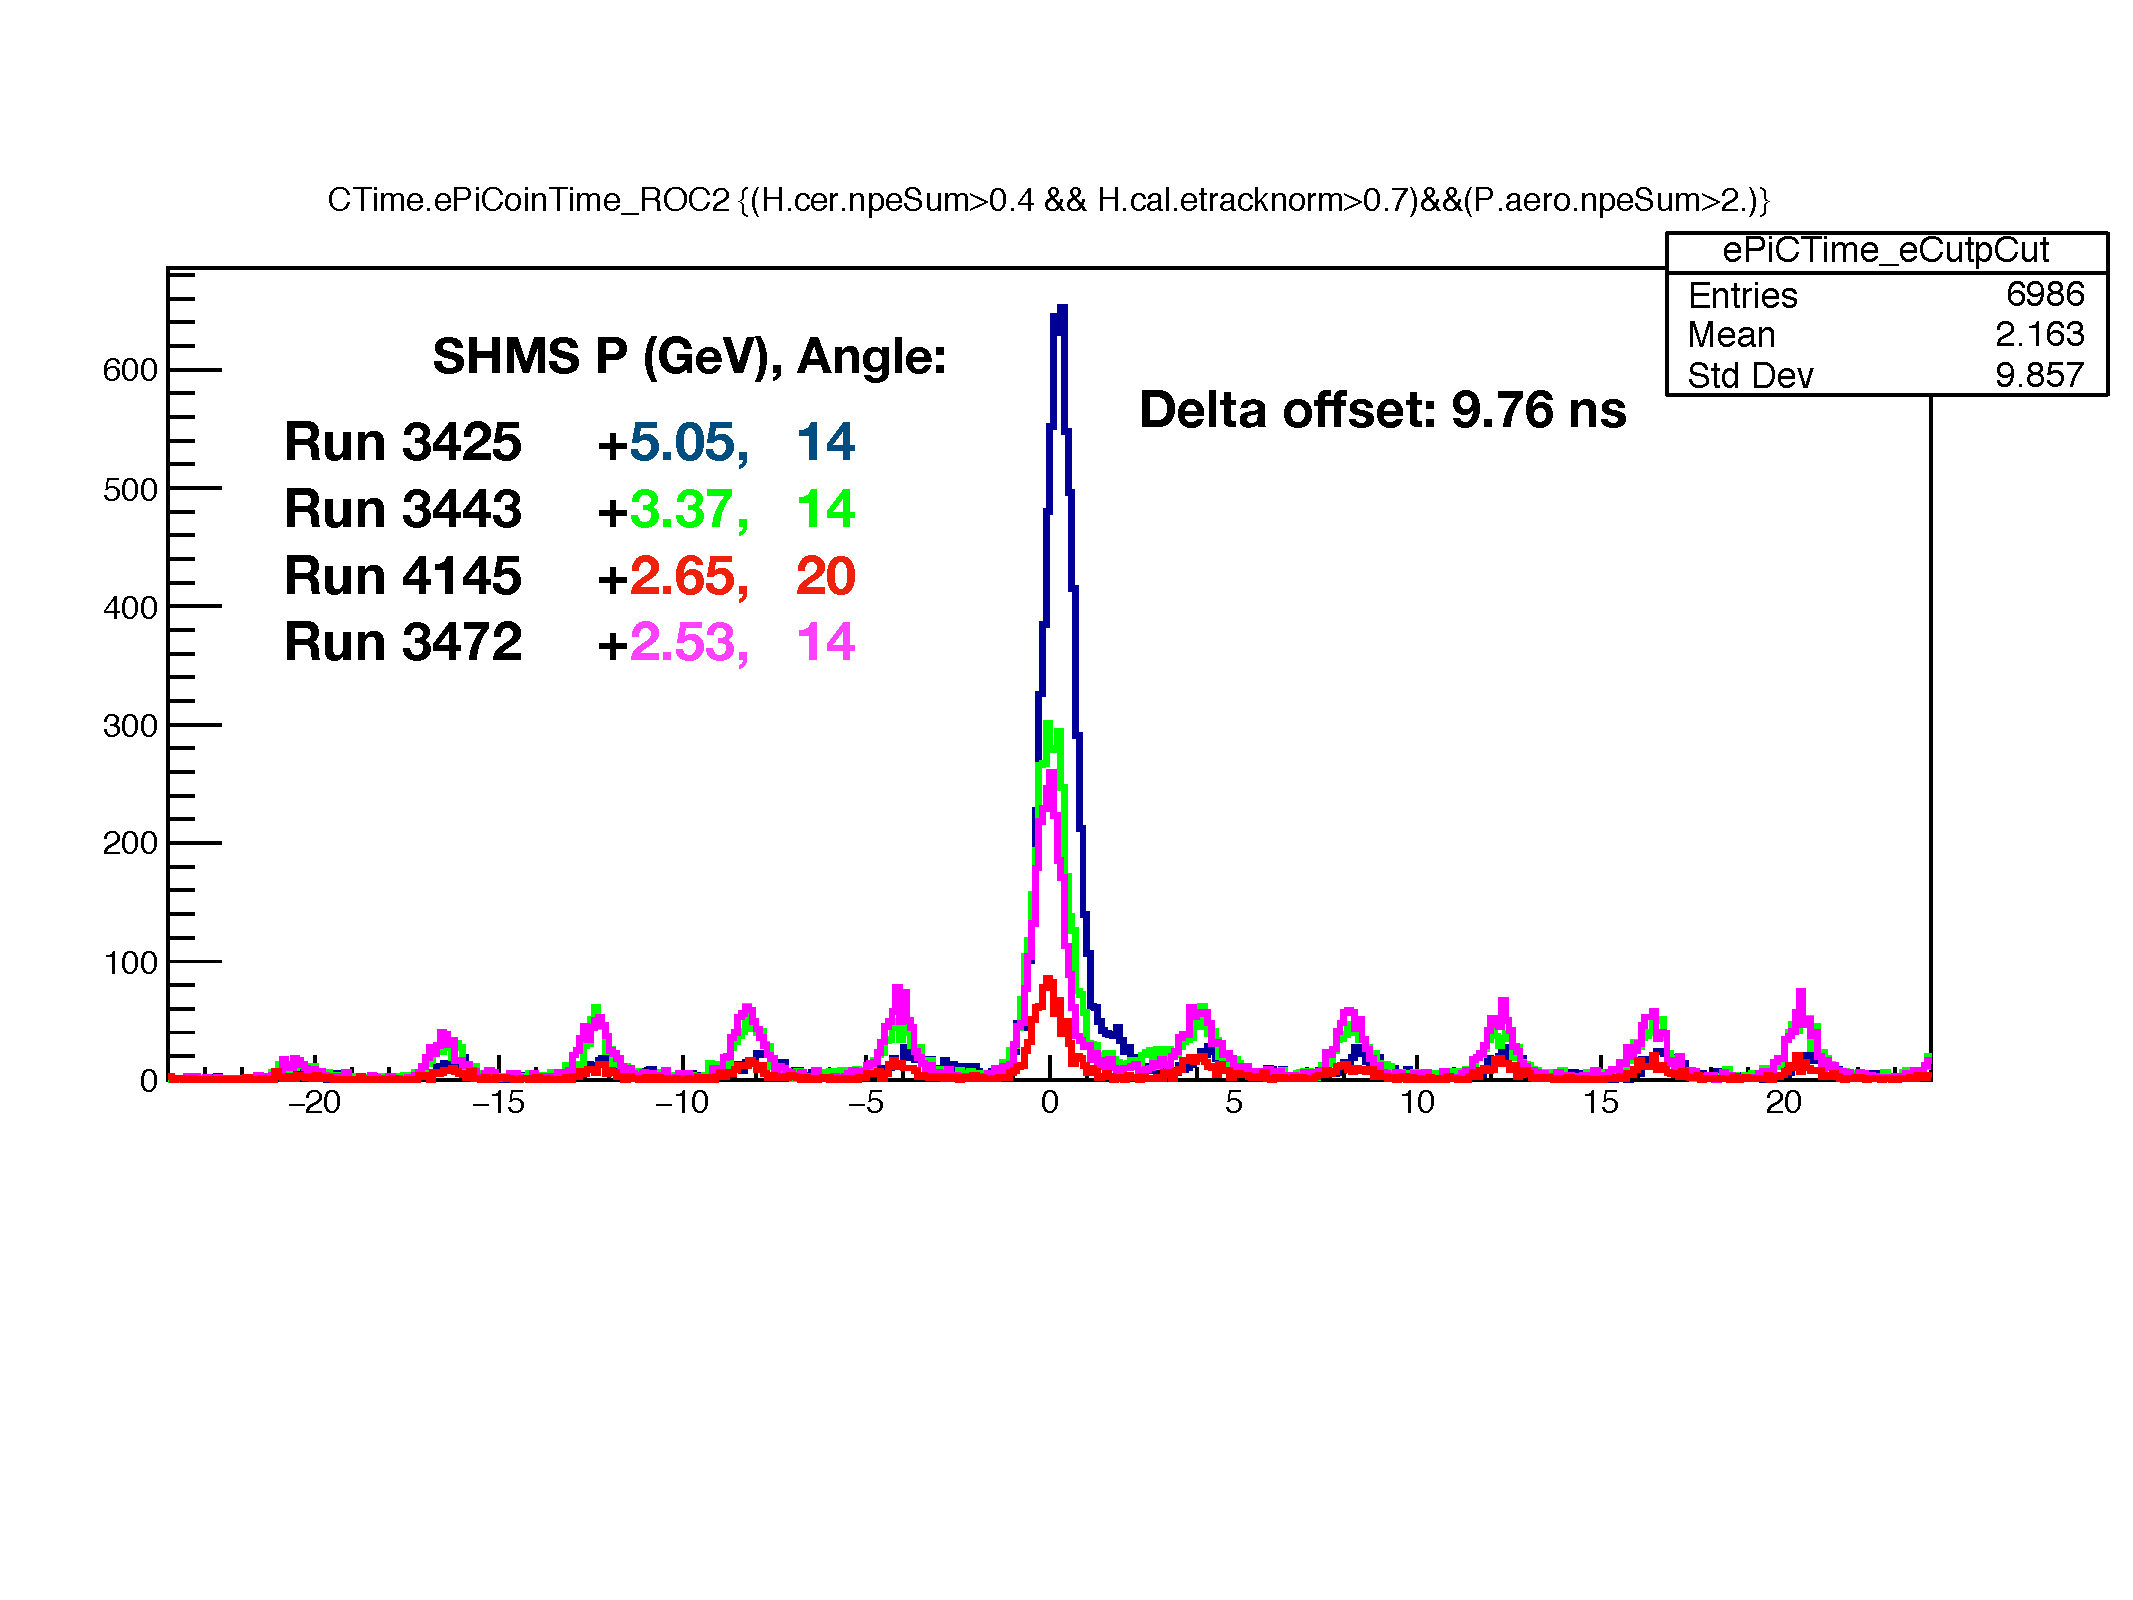
\includegraphics[scale=0.5]{ePi_compare.pdf}
  \caption{e$\pi^{+}$ coincidence time, assuming pion mass. A $\delta_{\text{offset}}$ has been determined and applied to several SIDIS runs.}
  \label{fig:eH_offset}
  \end{figure}
  \\
  \noindent A $\delta_{\text{offset}}$ of 9.76 ns was determined from SIDIS run 4145, using clean e$^{-}\pi^{+}$ coincidences. A calorimeter and Cherenkov cut was
  applied on the HMS for selecting electrons, and an Aerogel photoelectron cut was applied on the SHMS
  to eliminate proton contamination showing up in the accidentals. After obtaining a clean sample of e$^{-}\pi^{+}$ coincidences, a fit was done to the main peak to
  determine the offset. The stability of the offset was tested for various SIDIS runs at different SHMS momenta. (See Figure \ref{fig:eH_offset})

  \newpage

  \section{Discussion on Coincidence Time Module Workflow}
  \noindent The coincidence time physics module can be found under hcana/src directory, with the name of \texttt{THcCoinTime.cxx(.h)}. The module
  is a derived class from more general Hall A class \texttt{THaPhysicsModule.C(.h)}, and hence, it also uses all of its member functions/methods. The
  class is called in the main Hall C analysis coincidence replay scripts, located in: \\
  \texttt{/hallc\_replay/SCRIPTS/COIN/PRODUCTION/}. I will start by discussing how the physics module is calle in the analyzer, and then
  briefly discuss the relevant methods used for calculating the coincidence time in chronological order.
  
  \begin{lstlisting}[language=C++, caption={Adding the Module in the Analyzer}] 
    void replay_production_coin_hElec_pProt(Int_t RunNumber = 0, Int_t MaxEvent = 0) {
     
      //A few lines later, towards the end of the code (line # are not same) 
      //This replay script is in: /hallc_replay/SCRIPTS/COIN/PRODUCTION/
      
      THcCoinTime* coinTime = new THcCoinTime("CTime", "Coincidence Time Determination",
      "P", "H", "T.coin"); 
      gHaPhysics->Add(coinTime);

    }
  \end{lstlisting}
  In the snippet of code above (Listing 1), an instance (coinTime) of the class is created and initialized with arguments that will be used
  later on. The order in which the arguments ``P" and ``H" are called is important, as they dictate which spectrometer will be the electron or hadron arm,
  an so they must be consistent with the replay script that is called. \\
  \newline
    \begin{lstlisting}[language=C++, caption={THcCoinTime.cxx, The Constructor Method}] 
      THcCoinTime::THcCoinTime (const char *name, const char* description,
      const char* hadArmName, const char* elecArmName, const char* coinname) :
  
  THaPhysicsModule(name, description), 
  fCoinDetName(coinname), 
  fhadArmName(hadArmName),                 //initialize spectro names
  felecArmName(elecArmName),
  fhadSpectro(NULL),                      //initialize spectro objects
  felecSpectro(NULL),
  fCoinDet(NULL)
{

}

  \end{lstlisting}

\noindent In the Listing 2 snippet above, the constructor is defined with some arguments, which were called in Listing 1. The first argument, \textit{name},
represents the name of the class and will be the \textit{prefix-} in every ROOT leaf variable that is added in the DefineVariables() method. The
third and fourth arguments, take the char value ``P" or ``H", depending on which spectrometer will be the hadron/electron arm. The arguments in
the constructor are paseed on in lines 4-7. Additional \texttt{THcHallCSpectrometer.cxx} objects are initialized in lines 8-10, and will be used later on.\\


\begin{lstlisting}[language=C++, caption={THcCoinTime.cxx, The Init() Method}] 
  THaAnalysisObject::EStatus THcCoinTime::Init( const TDatime& run_time )
  {
    // Initialize THcCoinTime physics module

  fhadSpectro = dynamic_cast<THcHallCSpectrometer*>
    ( FindModule( fhadArmName.Data(), "THcHallCSpectrometer"));
  if( !fhadSpectro ) {
    cout << "THcCoinTime module  Cannnot find Hadron Arm = " <<  fhadArmName.Data() << endl;
    fStatus = kInitError;
    return fStatus;
  }

  //The other two objects are also casted, but due to space, were not included.
  
\end{lstlisting}
In the \texttt{Init()} method above, the objects initialized to NULL in the constructor are converted to
\texttt{THcHallCSpectrometer} objects via a \texttt{dynamic\_cast}, which enables the object to use all member functions
of mentioned class. \\

\begin{lstlisting}[language=C++, caption={THcCoinTime.cxx, The ReadDatabase() Method}] 
Int_t THcCoinTime::ReadDatabase( const TDatime& date )
{
  // Read database. Gets variable needed for CoinTime calculation


  DBRequest list[]={
    {"eHadCoinTime_Offset",  &eHad_CT_Offset, kDouble, 0, 1},  
    {"HMS_CentralPathLen",  &HMScentralPathLen, kDouble, 0, 1},
    {"SHMS_CentralPathLen", &SHMScentralPathLen, kDouble, 0, 1},
    {0}
  };
  
  //Default values if not read from param file
  eHad_CT_Offset = 0.0;

  HMScentralPathLen = 22.0*100.;
  SHMScentralPathLen = 18.1*100.;

  
  gHcParms->LoadParmValues((DBRequest*)&list, "");

  return kOK;
}
\end{lstlisting}
The \texttt{ReadDatabase()} method searches for a \texttt{coincidence time offset} and \texttt{SHMS/HMS Path Length}
parameters. The \texttt{coincidence time offset} parameter is located in \texttt{/PARAM/TRIG/tcoin.param}, and the
\texttt{SHMS/HMS Path Length} parameters are located in  \texttt{/PARAM/SHMS/GEN/pcana.param} and
\texttt{/PARAM/HMS/GEN/hcana.param} directories, respectively. In the scenario that any of the above parameters
were NOT found, they would be initialized by default under this method. (See line \# 14, 16 and 17 of this method)
\\
\begin{lstlisting}[language=C++, caption={THcCoinTime.cxx, The Process() Method}] 
Int_t THcCoinTime::Process( const THaEvData& evdata )
{
  
 //Create THaTrack object for hadron/elec arms to get relevant golden track quantities
  if (felecArmName=="H") {
    theSHMSTrack =(fhadSpectro->GetGoldenTrack());     
    theHMSTrack = (felecSpectro->GetGoldenTrack());
  } else{
    theSHMSTrack =(felecSpectro->GetGoldenTrack()); 
    theHMSTrack = (fhadSpectro->GetGoldenTrack());
  }
  //Gather relevant variables for Coincidence time calculation
  lightSpeed = 29.9792; // in cm/ns

  //Particle Masses (HardCoded)
  elecMass =  0.510998/1000.0; // electron mass in GeV/c^2
  positronMass =  0.510998/1000.0;
  protonMass = 938.27208/1000.0; // proton mass in GeV/c^2	
  kaonMass = 493.677/1000.0;    //charged kaon mass in GeV/c^2
  pionMass = 139.570/1000.0;    //charged pion mass in GeV/c^2

  
      //SHMS arm
      Double_t shms_xptar = theSHMSTrack->GetTTheta();     
      Double_t shms_dP = theSHMSTrack->GetDp();            
      Double_t SHMS_FPtime = theSHMSTrack->GetFPTime();    
      
      //HMS arm
      Double_t hms_xfp = theHMSTrack->GetX();           
      Double_t hms_xpfp = theHMSTrack->GetTheta();      
      Double_t hms_ypfp = theHMSTrack->GetPhi();        
      Double_t HMS_FPtime = theHMSTrack->GetFPTime();    
      
      //Get raw TDC Times for HMS/SHMS (3/4 trigger)
      pTRIG1_rawTdcTime_ROC1 = fCoinDet->Get_pTRG1_ROC1_rawTdctime(); 
      pTRIG4_rawTdcTime_ROC1 = fCoinDet->Get_pTRG4_ROC1_rawTdctime();
      pTRIG1_rawTdcTime_ROC2 = fCoinDet->Get_pTRG1_ROC2_rawTdctime();
      pTRIG4_rawTdcTime_ROC2 = fCoinDet->Get_pTRG4_ROC2_rawTdctime();

	  DeltaSHMSpathLength = -0.11*atan2(shms_xptar,1)*1000 - 0.057*shms_dP;
	  DeltaHMSpathLength = 12.462*hms_xpfp + 0.1138*hms_xpfp*hms_xfp - 0.0154*hms_xfp
          - 72.292*hms_xpfp*hms_xpfp - 0.0000544*hms_xfp*had_xfp - 116.52*hms_ypfp*hms_ypfp;

          // default assume SHMS is electron arm
	  Double_t ElecPathLength=SHMScentralPathLen +  DeltaSHMSpathLength;
	  Double_t HadPathLength=HMScentralPathLen +  DeltaHMSpathLength;

          elec_P = theSHMSTrack->GetP();     //electron golden track arm momentum
          had_P = theHMSTrack->GetP();       //hadron golden track arm momentum

          Int_t sign=-1;

          if (felecArmName=="H") {
             ElecPathLength=HMScentralPathLen +  DeltaHMSpathLength;
	     HadPathLength=SHMScentralPathLen +  DeltaSHMSpathLength;
             elec_P = theHMSTrack->GetP();    //electron golden track arm momentum
             had_P = theSHMSTrack->GetP();    //hadron golden track arm momentum
             sign=1;
	  }

	  //beta calculations beta = v/c = p/E
	  elecArm_BetaCalc = elec_P / sqrt(elec_P*elec_P + elecMass*elecMass);
	  hadArm_BetaCalc_proton = had_P / sqrt(had_P*had_P + protonMass*protonMass);


	  //Coincidence Corrections
	  elec_coinCorr = (ElecPathLength) / (lightSpeed * elecArm_BetaCalc );
	  had_coinCorr_proton = (HadPathLength) / (lightSpeed * hadArm_BetaCalc_proton );

	  //Raw, Uncorrected Coincidence Time
	  fROC1_RAW_CoinTime =  (pTRIG1_rawTdcTime_ROC1*0.1 + SHMS_FPtime)
          - (pTRIG4_rawTdcTime_ROC1*0.1 + HMS_FPtime);

	  //Corrected Coincidence Time for ROC1/ROC2 (ROC1 Should be identical to ROC2)
	  //PROTON
	  fROC1_epCoinTime = fROC1_RAW_CoinTime + sign*( elec_coinCorr-had_coinCorr_proton)
          - eHad_CT_Offset;    
  
  
  return 0;

}
\end{lstlisting}
The coincidence time calculations are done in the Process() method. It may be
non-trivial to follow everything that is done here, so I will attempt to summarize
it based on the code line numbers.
\begin{itemize}
\item Lines 4-10: Based on whether the electron arm is set to HMS("H") or SHMS("P"),
  then associate the \texttt{GetGoldeTrack()} method with either \texttt{THaTrack.cxx}
  objects for HMS or SHMS. The quantities necessary to do the calculations can then
  be obtained from \texttt{theSHMSTrack} or \texttt{theHMSTrack THaTrack.cxx} objects. 
\item Lines 23-33: The relevant HMS/SHMS variables to be used in the Path Length correction
  are obtained from the track objects mentioned in the first bullet.
\item Lines 34-38: Call functions to get the raw TDC Time from each spectrometer
  single arm triggers, \texttt{pTRIG1(3/4 SHMS)} and \texttt{pTRIG4(3/4 HMS)}. The
  \texttt{fCoinDet} object is an instance of the \texttt{THcTrigDet.cxx} class,
  and calls methods to get these raw times, which had to be added in the abovementioned
  class during the time this module was created.
\item Lines 44-60: Start with the assumption that the SHMS is the electron arm,
  determine the corrected path length and golden track momentum, and most importantly,
  define the sign of the correction to be -1, so that the correction to the
  electron/hadron arms is actually subtracted from the raw times, and eliminating any
  dependence of the coincidence time on the particle type. If the electron arm is the
  HMS, then the corrected path length, golden track momentum and the sign invert roles
  between spectrometers.
\item Lines 61-78: Once the electron and hadron arm are associated with a spectrometer,
  then lines 62-63 determine the velocity of the electron and hadron. (I only included
  the Proton, but the calculation was also done for Kaons, Pions and Positrons.)
  Lines 67-68 determine the time it takes the particle to traverse through the spectrometer
  into the focal plane. Lines 71-72 determine the raw coincidence times by taking the
  difference between the raw TDC times determined in Lines 35-38. The focal plane times
  are also included here, so simplify the calculation later on. Finally, Lines 76-77
  combine the elements in Lines 66-72, along with the sign, to determine the corrected
  coincidence time. An offset is added towards the end in order to shift the coincidence peak
  to zero. This offset is read as a parameter in the \texttt{ReadDatabase()} method.
  
\end{itemize}
    




% --------------------------------------------------------------
%     You don't have to mess with anything below this line.
% --------------------------------------------------------------
 
\end{document}
